\documentclass[11pt,a4paper]{article}
\usepackage{import}
\subimport{../../shared/}{preamble.tex}
\addbibresource{bibliography/references.bib}
\title{Gradient Fitting of a Common Co-Energy Potential for dq Flux Reconstruction}
\author{}
\date{7 October 2026}
\newcommand{\PaperAbstract}{Can inconsistent flux samples be represented by slopes of a common scalar potential? A differentiable symmetric B-spline potential gives a linear gradient fit with gauge fixing and a penalty on changing curvature. Integrability and reflection hold by construction. Controlled synthetic experiments distinguish flux accuracy, Hessian accuracy and exact structural guarantees. A portable real PSM demonstration compares independent, parity-only and potential fits on spatially withheld regions, with raw values and discarded residuals preserved. The real constrained fits incur larger prediction error against measured samples; enforced consistency is therefore a model restriction, not evidence of improved magnetic truth.}
\newif\ifshowglossary\showglossarytrue
\newif\ifshowbibliography\showbibliographytrue


\begin{document}
\maketitle
\begin{abstract}
\PaperAbstract
\end{abstract}
\tableofcontents

\section{Question and contribution}
Measured flux supplies slopes, not scalar energy observations. The question
is how to use all those slopes to reconstruct one consistent potential while
making the discarded information explicit. The contribution is a common
gradient fit with a gauge, symmetric basis and controlled curvature penalty,
evaluated separately on known synthetic fields and unknown real fields.

Energy-based motor models motivate a scalar storage representation
\cite{jebai2014}; nonlinear coupled flux models illustrate saturation and
reciprocity \cite{sun2020}. Here the basis is chosen for transparent derivative
coupling rather than a universal interpolation advantage. The companion
consistency study tests whether terminal-current samples actually admit the
declared model \cite{companion-consistency}. Even when they do not, a potential
fit defines a useful model projection, provided raw samples and residuals
remain part of the reported result.

\section{Model class and coordinate normalization}
\label{sec:potential}
On a fixed quasi-static state, assume a differentiable scalar landscape with
\begin{equation}
 \flux=\nabla_{\current}\coenergy,\qquad
 \coenergy(i_d,i_q)=\coenergy(i_d,-i_q).
 \label{eq:potential-gradient}
\end{equation}
The second condition is an additional reflection assumption. For a single
amplitude-invariant three-phase system $W'$ is physical co-energy divided by
$3/2$, so the gradient has the usual dq flux units.
Height is unobservable from slopes: $W'+C$ produces the same flux. Fix its
value at a supported reference as a gauge. The Hessian then supplies local
differential inductance, but the fit does not automatically establish
positive curvature or a true storage law in terminal-current coordinates.

Flux samples may be inconsistent with this class. Choosing a landscape whose
slopes best explain them is a projection under a basis, metric and regularizer.
Path integration is an alternative for exact conservative fields; with noisy
inconsistent data an arbitrary chosen path hides disagreement. The gradient
fit retains all sample directions and their residuals instead.

\section{Fit a common scalar potential directly in the gradient domain}
Two independent approximations $\psi_d=f_d(i_d,i_q)$ and
$\psi_q=f_q(i_d,i_q)$ can have low sample error without correct parity or
integrability. Even parity-constrained independent fits do not guarantee a
common potential: $f_d=1+i_q^2$, $f_q=i_q$ have the required parities but
mixed derivatives $2i_q$ and zero. The missing information is the coupling
between their slopes.

The physically structured representation is
\begin{equation}
 \boxed{\hat\flux_{\rm fit}=\nabla\hat\coenergy,\qquad
 \hat\coenergy(i_d,i_q)=\hat\coenergy(i_d,-i_q).}\label{eq:fit-potential}
\end{equation}
A $C^2$ even scalar basis guarantees flux parity by the chain rule and
reciprocity by equality of mixed derivatives. Saturation and cross-saturation
are retained in the variation of its Hessian, not removed by symmetry.
The potential ties both flux surfaces to the same source of curvature.

Let $\vect c$ be its coefficients and $\vect\psi_k^{\rm rec}$ reconstructed
samples. The basic fitting problem is
\begin{equation}
 \boxed{\min_{\vect c}\sum_k
 \norm{\nabla\coenergy(\current_k;\vect c)-\vect\psi_k^{\rm rec}}^2
       +\lambda\mathcal R(\coenergy),\quad \coenergy(\current_0)=0.}
 \label{eq:gradient-fit}
\end{equation}
This asks for the admissible scalar landscape whose slopes best match the
observed vectors. It never requires directly measured energy samples.
If the terminal-current field is inconsistent with the declared magnetic
class, this minimization is a regularized projection onto that class under
the selected weights and basis. It does not establish a true storage law
in those terminal coordinates. Retain the sample residual
$\vect r_k=\vect\psi_k^{\rm rec}-\nabla\hat\coenergy(\current_k)$ alongside
predictions; constructed zero curl is not evidence that its discarded part
was entirely measurement error. Use
whitened residuals when uncertainties differ or share correlations; the
reconstruction divides voltage error by speed, so uniform flux uncertainty
should not be assumed across speeds.

Regularization controls degrees of freedom that measurements constrain weakly.
For example, a penalty on the spatial variation of the Hessian discourages
rapidly oscillating differential inductance. A penalty on the Hessian itself
also biases nonzero inductance toward zero; that distinction matters. Select
penalty strength using held-out regions and derivative targets, not training
error alone. Nondimensionalize current and flux so the numerical weight and
penalty have interpretable units. Robust losses may limit isolated outliers,
but cannot distinguish systematic bias from genuine magnetics.

Gauge removes the constant null direction. Additional rank deficiency can
remain if sample locations do not excite basis directions. Check the gradient
design rank on the gauge-fixed subspace and inspect scaled singular values
\cite{horn2013}. A smooth fitted potential is not necessarily locally convex:
positive differential inductance requires a separate Hessian constraint or
an explicit check over the supported domain.

\section{Numerical realization: a symmetric B-spline potential}
\subsection{Construct even basis functions rather than repair fitted maps}
Scale coordinates to $x=i_d/I_*$ and $y=i_q/I_*$, and approximate
$\coenergy=\psi_*I_*\normalizedcoenergy$. On symmetric q knots, define paired basis functions
\begin{equation}
 E_n(y)=\tfrac12\bigl(B_n(y)+B_n(-y)\bigr),\qquad
 \normalizedcoenergy(x,y)=\sum_{m,n}c_{mn}B_m(x)E_n(y).\label{eq:spline-potential}
\end{equation}
Keep one representative of each reflected pair to avoid duplicated columns.
Then $E_n$ is even, $E'_n$ is odd, and $E''_n$ even. Analytic differentiation
gives
\begin{align}
 \psi_d/\psi_*&=\sum c_{mn}B'_mE_n,&
 \psi_q/\psi_*&=\sum c_{mn}B_mE'_n,\\
 L_{dd}/L_*&=\sum c_{mn}B''_mE_n,&
 L_{dq}/L_*&=L_{qd}/L_*=\sum c_{mn}B'_mE'_n,\\
 L_{qq}/L_*&=\sum c_{mn}B_mE''_n,&L_*&=\psi_*/I_*.
\end{align}
The structural properties now hold by construction, including between samples.
Differential inductance is surface curvature; its change across the current
plane expresses saturation and cross-saturation.

For degree $p$ with simple interior knots a spline is $C^{p-1}$ there.
A cubic potential therefore has continuous Hessian but its third derivatives
can jump at knots. The illustration uses degree four to obtain continuous
third derivatives at simple interior knots. Repeated knots reduce continuity;
the intended derivative quality must guide knot multiplicities. Local support
limits the number of active coefficients per sample. The standard B-spline
definition and analytic derivatives are documented in \cite{scipy-bspline}.

\subsection{A linear gradient design and regularization}
Each sample adds two rows $[B'_mE_n]$ and $[B_mE'_n]$ to a design matrix
$\matr G$. The normalized data stack is $\vect z$. With a roughness operator
$\matr P$, solve
\begin{equation}
 \min_{\vect c}\norm{\matr G\vect c-\vect z}^2
          +\lambda\norm{\matr P\vect c}^2,
 \qquad \vect g_0\trans\vect c=0.\label{eq:spline-solve}
\end{equation}
Here $\vect g_0$ evaluates the potential at the reference. A null-space basis
of the gauge row gives an unconstrained least-squares problem in fewer
variables. QR or SVD exposes residual rank deficiency without forming a
poorly conditioned normal matrix. For the synthetic experiment $\matr P$
samples $\normalizedcoenergy_{xxx},\sqrt3\normalizedcoenergy_{xxy},\sqrt3\normalizedcoenergy_{xyy},\normalizedcoenergy_{yyy}$ on a uniform grid,
with quadrature weights. It approximates the squared norm of the third
derivative tensor and penalizes changing Hessian rather than constant inductance.

\subsection{Alternative representations and what they guarantee}
Independent unconstrained RBF surfaces can accommodate scattered data but
enforce neither parity nor integrability by default. Independent even/odd
flux bases enforce parity but leave the mixed derivatives unrelated.
A scalar symmetry-aware RBF potential fitted through its gradients enforces
both, like the spline potential, if the basis is sufficiently differentiable.
RBF kernel shape, smoothing, polynomial augmentation, conditioning, and
support all require tuning; the standard interpolation interface documents
these numerical choices \cite{scipy-rbf}. No universal optimal basis is claimed.

\begin{table}[tb]
\centering\small
\begin{tabularx}{\textwidth}{@{}lYY@{}}
\toprule
Representation & Structural guarantee & Remaining numerical questions\\
\midrule
Independent flux RBFs & None by default & Kernel/shape, smoothing, conditioning,
derivatives, boundary support\\
Independent parity fits & d-even and q-odd & Reciprocity, derivative quality,
sample coverage, regularization\\
Common symmetric potential & Parity and reciprocity for a smooth basis &
Gradient-design rank, gauge, bias, curvature, convexity, tuning\\
\bottomrule
\end{tabularx}
\caption{Structural comparison. Guarantees do not establish which method has
the smallest prediction error on a particular measured data set.}
\end{table}
The small numerical comparison below uses B-splines for all three structural
classes to isolate constraints from kernel selection. RBF comparison remains
conceptual in this draft; a broad interpolator benchmark is separate work.

\section{Synthetic evaluation: sample error and physical structure}
\label{sec:synthetic}
\subsection{A known nonlinear field and distinct fitting experiments}
Let $I_*=\SI{100}{\ampere}$, $\psi_*=\SI{0.1}{\weber}$, and
$L_*=\psi_*/I_*=\SI{1}{\milli\henry}$. With $x=i_d/I_*$, $y=i_q/I_*$,
and $\coenergy=\psi_*I_*\normalizedcoenergy$, use
\begin{equation}
 \normalizedcoenergy=x+0.3x^2+0.5y^2
      -s(0.01x^4+0.02y^4)-0.03x^2y^2+0.02xy^2.
 \label{eq:synthetic-energy}
\end{equation}
Here $s=1$ is the baseline and $s=3$ strengthens d/q saturation. PM flux,
nonlinear self-saturation, and reciprocal cross-saturation are all present.
The normalized flux components are
\begin{align}
 \psid/\psi_*&=1+0.6x-0.04s x^3-0.06xy^2+0.02y^2,\\
 \psiq/\psi_*&=y-0.08s y^3-0.06x^2y+0.04xy,
\end{align}
with Hessian
\begin{equation}
 \Ldiff/L_*=
 \begin{bmatrix}
 0.6-0.12s x^2-0.06y^2&-0.12xy+0.04y\\
 -0.12xy+0.04y&1-0.24s y^2-0.06x^2+0.04x
 \end{bmatrix}.
\end{equation}
On $[-1,1]^2$, even at $s=3$, both diagonals are at least $0.18$ and
the off-diagonal magnitude at most $0.16$. Strict diagonal dominance proves
positive definiteness with eigenvalues at least $0.02$. This local polynomial
should not be extrapolated to arbitrarily large currents.

The experiment treats reconstructed flux samples as data with independent
normalized Gaussian noise of standard deviation $0.005$ per component. It
does not inject resistance or angle errors; those are the companion's
experiments. Draw scattered points uniformly on $[-1,1]^2$ using seed
20261006. Use 200 points for the noisy baseline, 50 for sparse sampling,
200 with five percent outliers for the outlier case, and 200 with $s=3$ for
stronger saturation. Outliers add Gaussian contamination of standard deviation
$0.1$ to both components of selected samples. No assertion about real sensor
noise is implied by this convenient synthetic distribution.

\subsection{Compare structural classes with the same spline family}
All candidates use degree-four B-splines with clamped endpoints at $-1,1$
and simple interior knots $-0.5,0,0.5$. Independent fits use two full tensor
bases. Parity fits use an even d basis and an odd q basis. The common potential
uses eight d basis functions and four even q basis functions: 32 coefficients,
31 after gauge fixing. Noiseless exact field recovery on a $13\times13$ sample
grid is checked separately; the chosen polynomial is representable in this
basis. This favorable approximation setting isolates noise and structure,
and limits conclusions about arbitrary machine maps.

Choose $\lambda$ among $0,10^{-6},10^{-5},10^{-4},10^{-3}$ using a fixed
80/20 split and validation flux error, then refit all samples with the selected
weight. Independent flux fits penalize their second derivatives, while the
potential fit penalizes third derivatives of co-energy, as described earlier.
These penalties target comparable flux smoothness but are not identical
optimization problems. The split is shared across candidates within each
case. One additional potential fit uses eight iteratively reweighted
least-squares steps with scalar Huber threshold $0.01$ for outliers.

Evaluate on a $25\times25$ grid over $[-0.95,0.95]^2$, distinct from the
training samples. Report componentwise flux RMSE in $\psi_*$ units, Hessian
entry RMSE in $L_*$ units, parity residual RMS in $\psi_*$ units, and curl
RMS in $L_*$ units. The evaluation avoids the exact outer boundary; it cannot
establish boundary or extrapolation reliability. Potential derivatives are
analytic basis derivatives, not numerical differences of interpolated flux.
\begin{table}[tbp]
\centering\scriptsize\begin{tabular}{llrrrr}
\toprule
Case & Fit & Flux RMSE & Hessian RMSE & Parity RMS & Curl RMS\\
\midrule
Noisy & Independent & 2.43e-03 & 1.40e-02 & 1.5e-03 & 2.2e-02 \\
Noisy & Parity & 1.81e-03 & 1.11e-02 & 0.0e+00 & 1.6e-02 \\
Noisy & Potential & 1.50e-03 & 1.24e-02 & 0.0e+00 & 0.0e+00 \\
Sparse & Independent & 6.80e-03 & 3.40e-02 & 4.7e-03 & 4.3e-02 \\
Sparse & Parity & 3.89e-03 & 1.79e-02 & 0.0e+00 & 2.5e-02 \\
Sparse & Potential & 2.87e-03 & 1.12e-02 & 0.0e+00 & 0.0e+00 \\
Outliers & Independent & 1.40e-02 & 8.26e-02 & 9.2e-03 & 1.0e-01 \\
Outliers & Parity & 1.03e-02 & 6.34e-02 & 0.0e+00 & 8.2e-02 \\
Outliers & Potential & 7.39e-03 & 4.74e-02 & 0.0e+00 & 0.0e+00 \\
Outliers & Potential robust & 1.50e-03 & 9.55e-03 & 0.0e+00 & 0.0e+00 \\
Strong saturation & Independent & 2.47e-03 & 1.98e-02 & 1.8e-03 & 1.7e-02 \\
Strong saturation & Parity & 1.85e-03 & 1.96e-02 & 0.0e+00 & 2.3e-02 \\
Strong saturation & Potential & 1.06e-03 & 7.91e-03 & 0.0e+00 & 0.0e+00 \\
\bottomrule
\end{tabular}

\caption{A single seeded illustrative experiment. Independent and parity
fits use flux B-splines; potential fits use co-energy gradients. Structural
zeros hold by construction. This is not an RBF benchmark or a statistical
ranking across many machines and sampling realizations.}
\label{tab:fit-metrics}
\end{table}

\subsection{What the numbers do and do not establish}
In the baseline, the potential fit has normalized flux RMSE about $0.00150$,
versus $0.00243$ for independent fits and $0.00181$ for parity fits.
Yet its Hessian RMSE is about $0.0124$, slightly higher than the parity fit's
$0.0111$. Better pointwise prediction therefore does not automatically mean
better derivatives. Selecting regularization only on flux error can underweight
the engineering importance of differential-inductance quality.

Parity fits eliminate forbidden reflection components but retain nonzero
curl. The common potential eliminates both structurally, even in noisy and
sparse cases. This is a representation guarantee, not evidence that every
remaining prediction is true. With outliers, the ordinary potential fit
still develops a negative minimum Hessian eigenvalue of approximately
$-0.0764$ on the evaluation grid. Energy consistency and symmetry alone do
not enforce positive differential inductance. The robust potential fit
reduces flux RMSE from approximately $0.00739$ to $0.00150$ and keeps positive
sampled eigenvalues in this realization. Grid positivity still does not prove
global positivity; an explicit convexity constraint would be a separate step.

The script verifies B-spline partition of unity and analytic derivative
recurrences, gauge, gauge-fixed rank, exact noiseless flux/Hessian recovery,
and structural parity and curl of fitted candidates. It stores metrics,
selected weights, and sampled Hessian eigenvalues in
\texttt{numerics/evaluation.json}. \begin{figure}[tbp]
\centering
\begin{tikzpicture}
\begin{groupplot}[group style={group size=2 by 2,horizontal sep=14mm,
 vertical sep=28mm},diagnostic axis,legend style={compact text,
 at={(.5,-.3)},anchor=north,legend columns=2}]
\nextgroupplot[title={d flux: slope along d},ylabel={$\psi_d/\psi_*$}]
 \addplot[reference quantity,strong line] table[x=y,y=dtrue]{figures/data/fit_slice.dat};
 \addlegendentry{True}
 \addplot[fitted curve] table[x=y,y=dfit]{figures/data/fit_slice.dat};
 \addlegendentry{Potential fit}
\nextgroupplot[title={q flux: slope along q},ylabel={$\psi_q/\psi_*$}]
 \addplot[reference quantity,strong line] table[x=y,y=qtrue]{figures/data/fit_slice.dat};
 \addplot[fitted curve] table[x=y,y=qfit]{figures/data/fit_slice.dat};
\nextgroupplot[title={d curvature},ylabel={$L_{dd}/L_*$}]
 \addplot[reference quantity,strong line] table[x=y,y=ddtrue]{figures/data/fit_slice.dat};
 \addplot[fitted curve] table[x=y,y=ddfit]{figures/data/fit_slice.dat};
\nextgroupplot[title={Mixed curvature},ylabel={$L_{dq}/L_*=L_{qd}/L_*$}]
 \addplot[reference quantity,strong line] table[x=y,y=dqtrue]{figures/data/fit_slice.dat};
 \addplot[fitted curve] table[x=y,y=dqfit]{figures/data/fit_slice.dat};
\end{groupplot}
\end{tikzpicture}
\caption{Baseline noisy-data potential fit at $x=-0.4$. Slopes and curvatures
come from the same fitted scalar surface. The fitted derivatives can show
visible error even when flux curves nearly coincide; parity and reciprocity
still hold structurally.}
\label{fig:fit-slice}
\end{figure}

These checks support reproducibility of
the illustration; they are not substitutes for varied-data validation.

\section{Real reconstruction as a model projection}
The 30-$^\circ$C reference slice of \texttt{psm\_temperature\_2500} supplies
340 OP means. True flux is unknown. Translate d current to its observed
midrange and scale d and q independently to the symmetric knot domain.
If $x_a=(i_a-c_a)/s_a$ and $W'=W_*\bar W$, physical flux is
$\psi_a=(W_*/s_a)\partial_{x_a}\bar W$. Thus gradient targets and predicted
derivatives include the anisotropic chain rule; an unscaled ordinate fit would
change the physical meaning of the Hessian. The numerical report stores all
centers and scales. The gauge-fixed gradient design has rank 31 of 31.

A deterministic spatial-bin fold with reflected q bins kept together leaves
267 training OPs and 73 held-out OPs. Only 61 held-out points lie inside the
training hull. Select the penalty among $0,10^{-6},10^{-5},10^{-4},10^{-3}$
using those supported points, then refit all samples. This tuning score is
not an independent final validation score; twelve unsupported locations are
not extrapolated for scoring. All three representations share the basis domain.

\begin{table}[htbp]\centering\small
\begin{tabular}{lrrrr}
\toprule
Fit & Tuning RMS & Sample RMS & Parity RMS & Curl RMS\\
\midrule
Independent & 0.573 & 0.437 & 2.543 & 0.037 \\
Parity & 2.646 & 2.583 & 0.000 & 0.010 \\
Potential & 2.713 & 2.647 & 0.000 & 0.000 \\
\bottomrule
\end{tabular}

\caption{Measured-sample comparison: tuning and full-sample RMS are in mWb;
curl RMS is in mH. Constructed zero structure is not a true-flux accuracy test.}
\end{table}
The constrained models predict the measured withheld values less closely.
They impose a hypothesis the real reconstruction does not exactly satisfy.
The common potential enforces zero curl, whereas parity alone leaves a curl
residual. Neither fact identifies the removed component as sensor error.
\begin{figure}[htbp]\centering
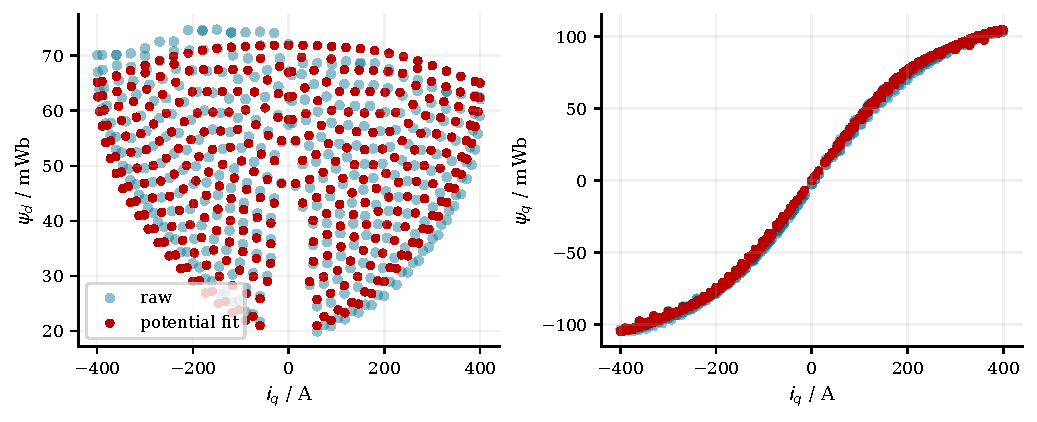
\includegraphics[width=\textwidth]{figures/real_reconstruction.pdf}
\caption{Raw and common-potential flux at each observed point, plotted against
q current. Points with different d current form distinct locations rather
than one fitted slice. Raw and reconstructed values are retained separately.}
\label{fig:real-reconstruction}\end{figure}
The full pointwise difference is exported as \texttt{real\_fit.csv}.
There is no extrapolation policy or experimental ground-truth correction claim.

\section{What the reconstruction guarantees and what it does not}
A smooth common potential couples derivatives everywhere in its model domain.
Its reciprocal mixed slopes and optional reflection do not depend on sample
fit error. Gauge removes a constant, while measured support and regularization
control additional weak directions. A full-rank design does not ensure good
conditioning, boundary accuracy, positive Hessian, or identifiable sensor bias.

Synthetic truth is representable in this basis and uses one seed, simple noise
and prescribed outliers. Its accuracy results do not establish a universal
winner. RBF alternatives are conceptual, not a numerical benchmark.
The real experiment has unknown magnetic truth and uses terminal currents,
nominal resistance and recorded electrical-speed/voltage channels. Its
spatial holdout reduces local leakage but selects the penalty on the reported
score. Additional independent campaigns and calibrated derivative references
would be needed for a physical accuracy claim.

The model predicts consistent slopes. The residual carries incompatible
measurements, excluded physical state, interpolation/basis error and penalty
bias together. Storage-coordinate qualifications are developed in the
companion consistency study \cite{companion-consistency}; here they are a
gate on interpretation rather than another fitting parameter.

\section{Conclusion}
A common scalar basis turns simultaneous flux reconstruction into a linear
gradient problem with an explicit gauge and curvature penalty. Synthetic tests
verify exact structural coupling while measuring flux and Hessian accuracy
separately. The real demonstration exposes the cost of enforcing the model:
larger measured-sample prediction error and an explicitly retained residual.
The method reconstructs a declared class; physical error correction requires
independent evidence for that class and for the removed contributions.


\ifshowglossary
  \glsadd{pmsm}\glsadd{dq}\glsadd{svd}
  \glsadd{sym:id}\glsadd{sym:iq}\glsadd{sym:rs}\glsadd{sym:omega}
  \glsadd{sym:ldiff}\glsadd{sym:coenergy}
  \printnoidxglossary[type=\acronymtype,title={Acronyms}]
  \printnoidxglossary[type=symbols,title={Symbols}]
\fi
\ifshowbibliography
  \printbibliography
\fi
\end{document}
